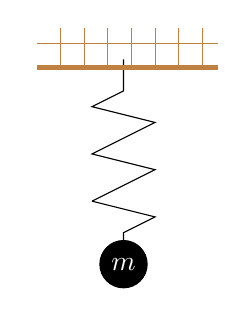
\begin{tikzpicture}

\draw [help lines, step=0.3cm, brown] (-1.5,1.5) node (v3) {} grid (0.8,2);


\draw (-0.4,1.6) -- (-0.4,1.2) -- (-0.8,1) -- (0,0.8) -- (-0.8,0.4) -- (0,0.2) -- (-0.8,-0.2) node (v1) {};
\draw (v1.center) -- (0,-0.4) -- (-0.4,-0.6) -- (-0.4,-1) node (v2) {};
\draw [fill] (v2) circle (0.3);
\node at (-0.4,-1) [white]{$m$};
\draw [ultra thick, brown](v3.center) -- (0.8,1.5);
\end{tikzpicture}